\documentclass[11pt]{article}
\usepackage[margin=18mm]{geometry}
\usepackage{booktabs,graphicx,hyperref}
\begin{document}
\title{Event analysis: selection and pad histories}
\author{NAUSICAA}\date{}\maketitle
The integrated checkpoint reads source-frame hits, produces rounded ion counts,
samples a common drift distance, diffuses each ion, and constructs Petit's kNN
graph. Events pass when exactly one component survives the configured ion
threshold. Accepted events supply their full retained diffusion table to pad
counting. The cumulative Julia suite passes 2016 assertions.

\section*{Selection and exact charge accounting}
\begin{center}\small\setlength{\tabcolsep}{4pt}
\begin{tabular}{lrrrrr}\toprule
Sample & Accepted/tested & Retained ions & Pad ions & Below cut, saved & Mean ms \\\midrule
Double beta & 22/50 & 2468695 & 2468695 & 7393 & 54.8 \\
Electron background & 31/50 & 3474395 & 3474395 & 14821 & 49.3 \\
\bottomrule\end{tabular}\end{center}
These events are a reproducible validation subset spread across each input file;
the acceptance fractions describe this subset. Retained and below-cut totals in
the table refer to accepted events. Every accepted event satisfies
$N_{\rm pads}=N_{\rm diffusion,retained}$ exactly. Rejected events retain their
decision and diffusion ledger. All events satisfy
$N_{\rm sampled}=N_{\rm retained}+N_{\rm outside}$ and
$N_{\rm retained}=N_{\rm graph}+N_{\rm below\ threshold}$.
Timings cover the computational pipeline after a warm-up, including allocations;
file reads and writes are outside the timed region.

\section*{Model and conventions}
The model retains the common-event thermal diffusion and per-hit rounding from
step two. Reconstruction cells have width $3\sigma_T$, maximum graph edges
$6\sigma_T$, and the configured nearest-neighbour count. The graph threshold is
applied to summed Int64 ion counts, inclusively; energies retain Petit's Float32
weights for the backbone. This gives exact equality at the configured threshold.

The selected track's energy-weighted x/y centre and minimum z define the grid
references, following Petit. Transverse grid edges receive one independently
sampled offset per axis in [0,pitch), shared by all slices. Whole-cell extensions
cover every retained diffusion-bin centre. All ions at a diffusion-bin centre
are assigned to its containing cell: this is the geometric collection
approximation. The independent physical pitch is read from the detector card.
Internal cells are half open; the final upper edge is included. Sparse pad
histories retain zero-count intervals through their complete saved axes.

The relative-time direction is increasing source z gives later arrival. The first arrival edge is t=0;
the sign and its source-z coordinate are saved with each history. Both signs are
supported. With 2 mm slices and 0.1 mm/ms drift, each slice is 20 ms. Absolute
event arrival offsets are a separate convention from these saved relative times.
Drift, diffusion and grid RNG streams use SHA-256 keys built from run seed,
sample, event ID and stage; event processing order preserves each stream.

\section*{Validation}
Tests cover Petit occupancy parity away from its excluded final boundaries,
exact threshold equality, disconnected-event rejection, full retained-charge
collection, grid extension, integer-pitch phase shifts, final edges, empty
histories, zero slices, both time directions and input ownership. An end-to-end
synthetic signal passes and a two-cloud background fails. Real-event replay is
identical; saved HDF5 histories are read back to check charge conservation.

\subsection*{Double beta; event 0}
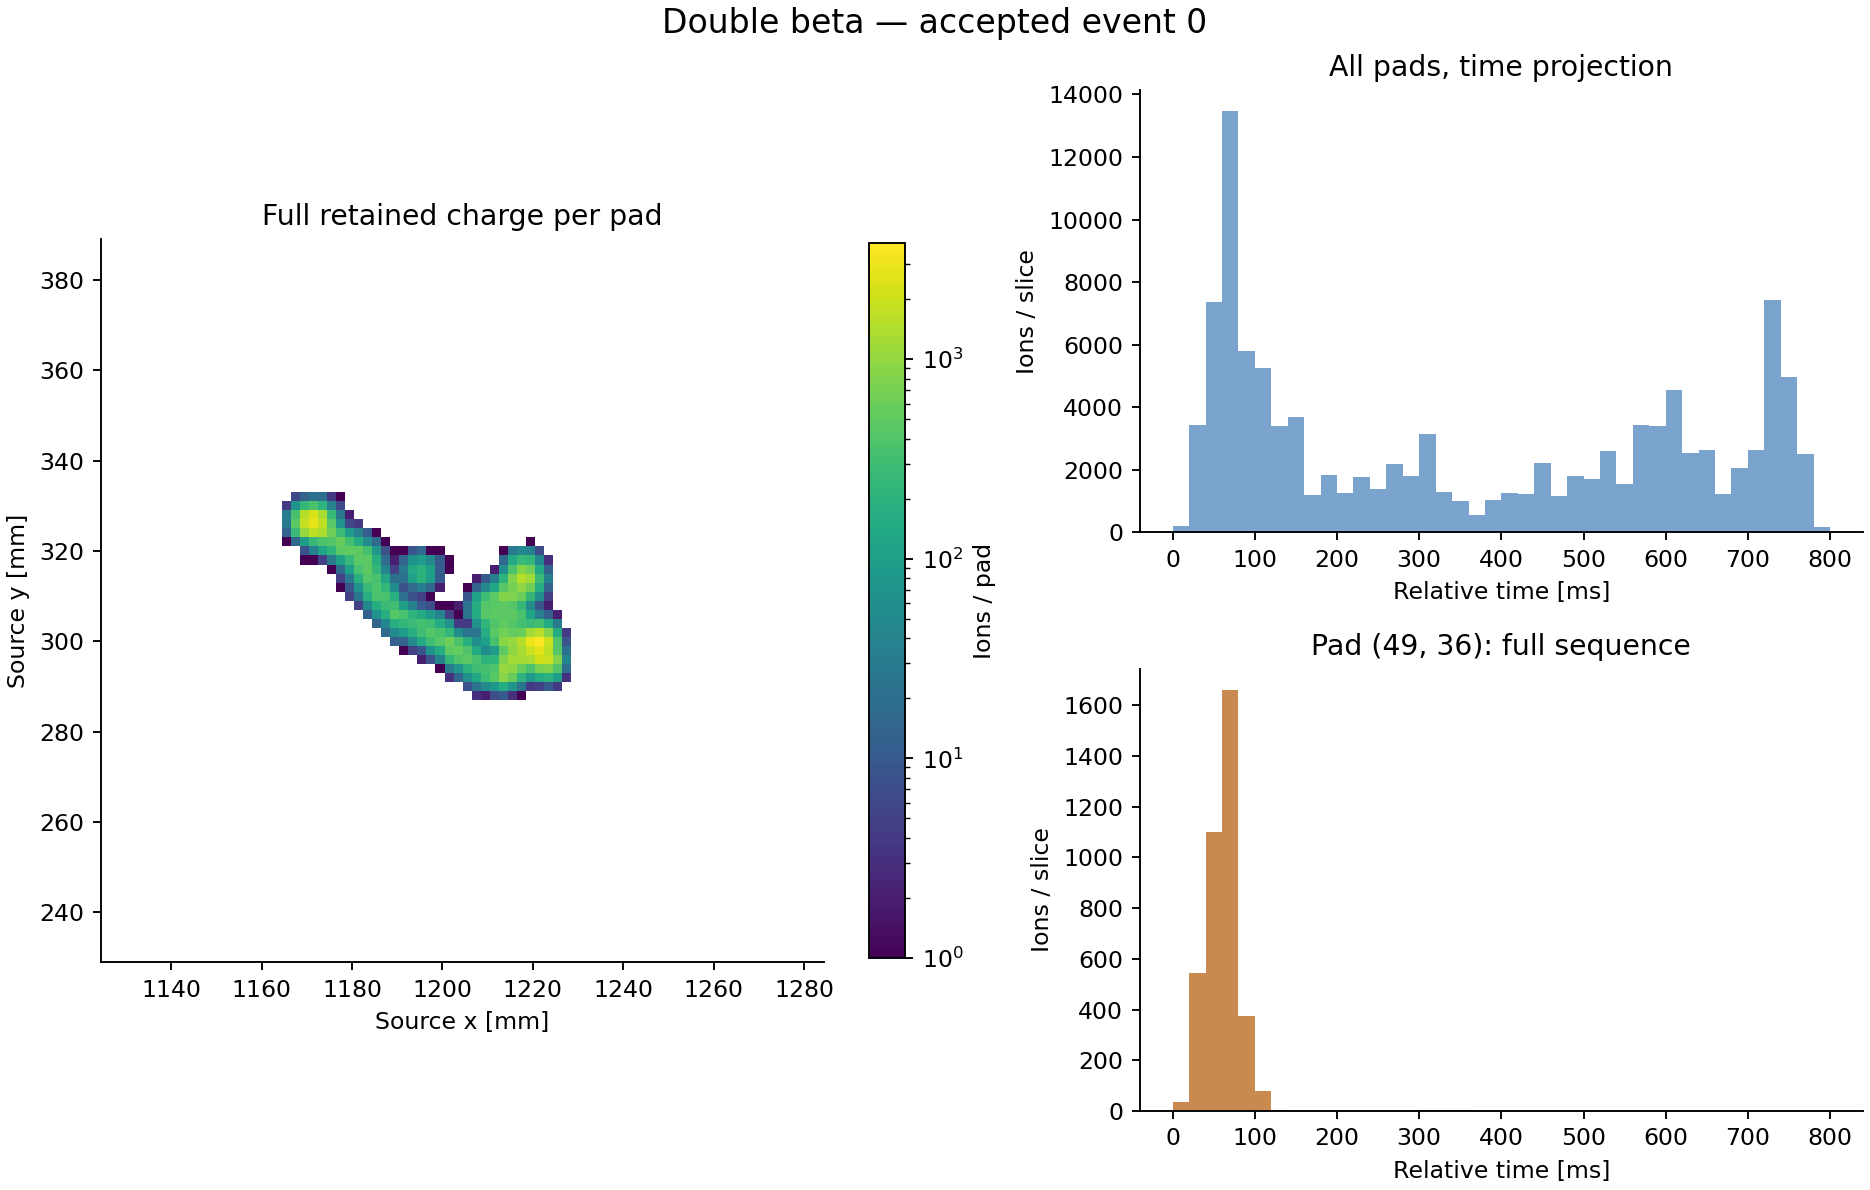
\includegraphics[width=\linewidth]{0nubb_pad_history.png}
\subsection*{Electron background; event 0}
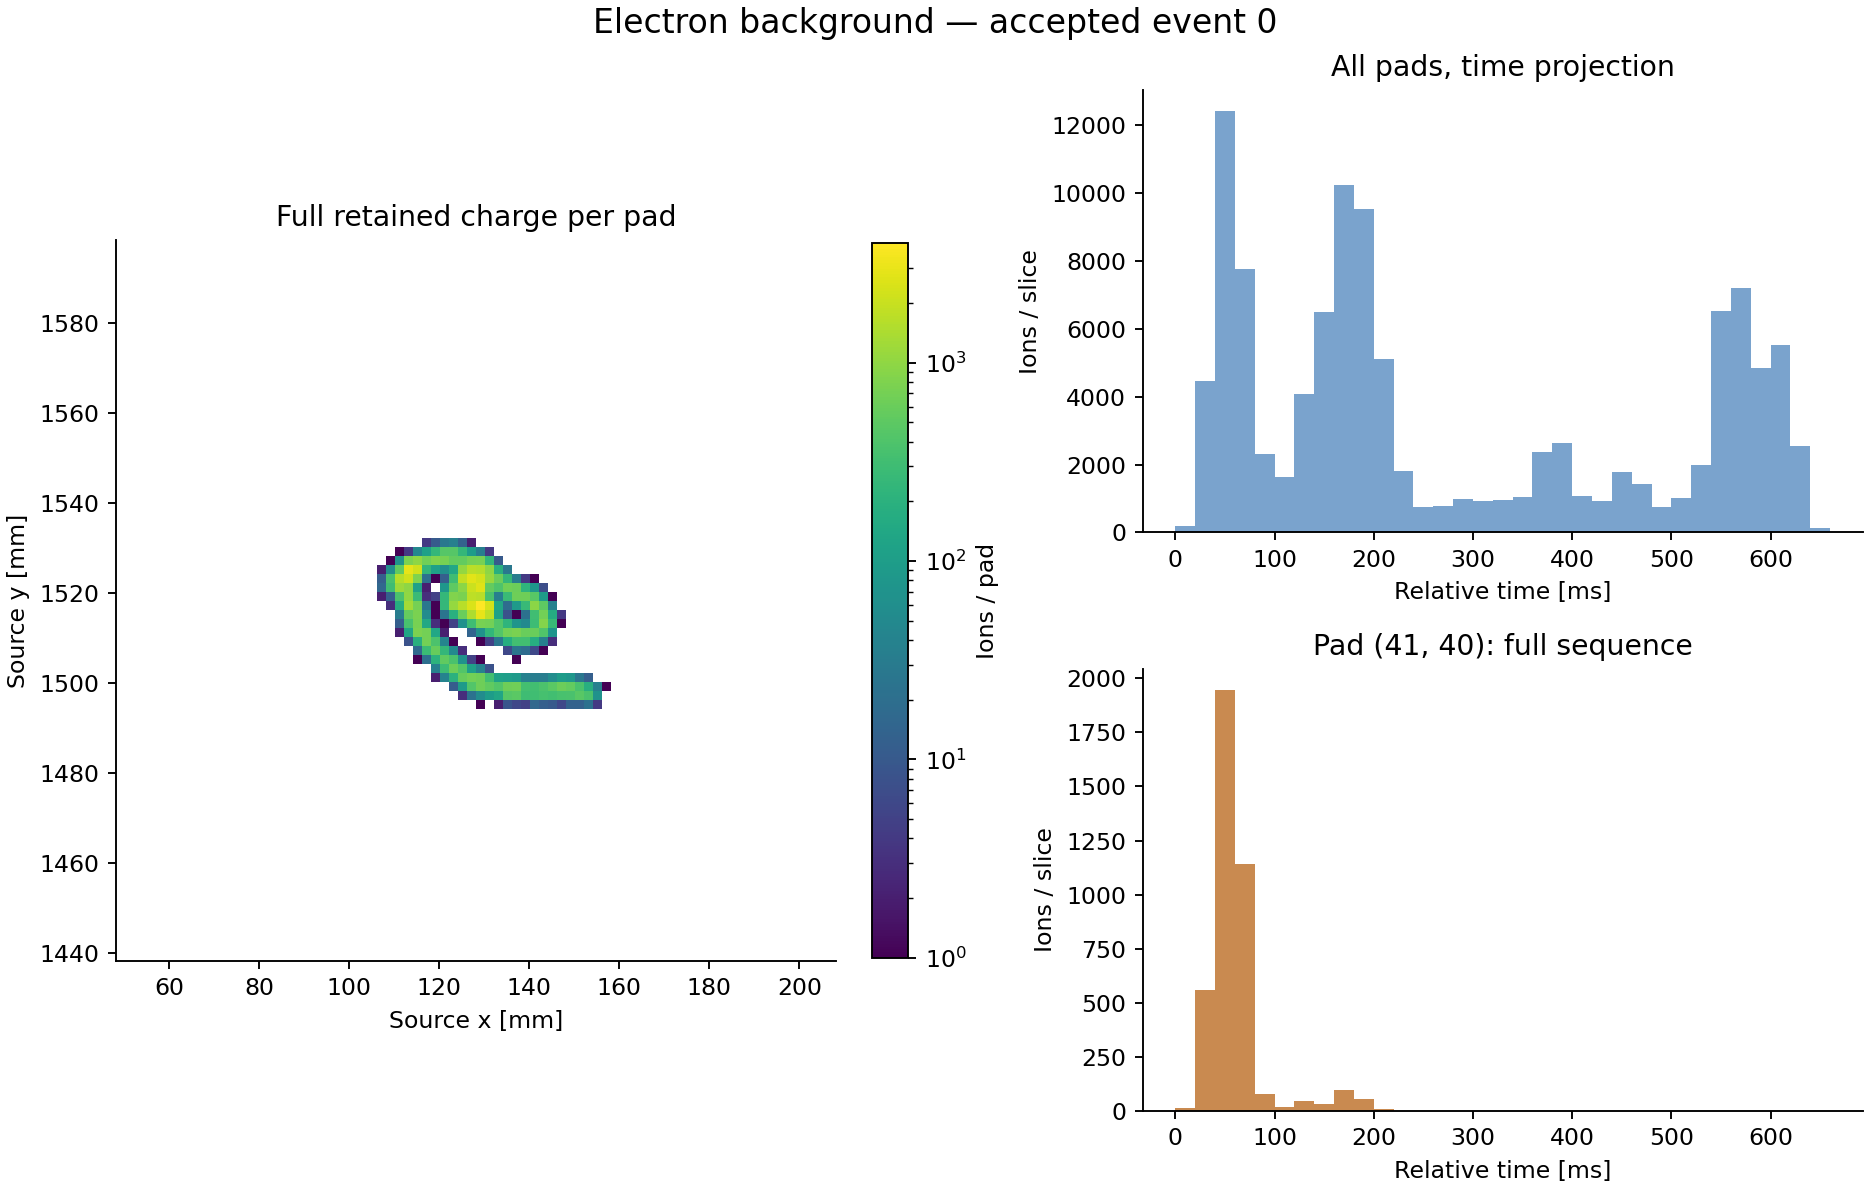
\includegraphics[width=\linewidth]{electron_0nubb_energy_pad_history.png}
\clearpage
\section*{Reproduction and next increment}
\begin{verbatim}
make validate-event-step3 PYTHON=/path/to/python3.11-or-newer
# Presentation only:
make report-event-step3 PYTHON=/path/to/python3.11-or-newer
\end{verbatim}
Numerical tables, histories, diffusion tables, axes, seeds and source hashes are in:
\par\noindent\path{results/event_analysis/step3_validation.h5}.
\par The next increment establishes the production output schema and common
ensemble axes/denominators, then runs parameter scans and the full samples.
\section*{Configuration used}
\footnotesize\begin{verbatim}
# Event-analysis checkpoints. Detector constants come from the SI card.
[inputs]
detector_card = "config/detector.toml"
samples = ["events/0nubb_hitdf.h5", "events/electron_0nubb_energy_hitdf.h5"]

[ionization]
ionisation_energy_eV = 21.9
# Same adopted nominal W as the initial ion_tracks analysis.

[drift]
min_cm = 10.0
max_cm = 150.0

[diffusion]
longitudinal = "thermal" # "zero" is the longitudinal comparison
nbins = 100
nsigma = 3.0

[graph]
method = "kNN"
k = 10
min_ions_per_bin = 10
bin_sigma_scale = 3.0
edge_sigma_scale = 6.0

[pads]
z_bin_width_mm = 2.0
minimum_xy_span_mm = 160.0
random_grid_offset = true
# Relative-time convention for this checkpoint: increasing z is later.
# Change to -1 for decreasing-z arrival order. t=0 is the first arrival edge.
drift_direction = 1
# Transverse pitch and ion speed are read from the detector card.

[random]
seed = 2026
# Validation uses explicit per-case seeds, stored in its HDF5.

[validation]
events_per_sample = 5
selection_events_per_sample = 50
synthetic_ions = 200000
drift_cm = [10.0, 80.0, 150.0]
bin_counts = [50, 100, 200]
padding_sigma = [2.0, 3.0, 4.0, 5.0]

\end{verbatim}
\end{document}
